% Sistemas de la relatividad especial: ejes (x,ct) ortogonales, (x',ct') inclinados (libro fig. 5.1)
\documentclass[border=4pt]{standalone}
\usepackage{tikz}
\usetikzlibrary{arrows.meta, calc}
\begin{document}
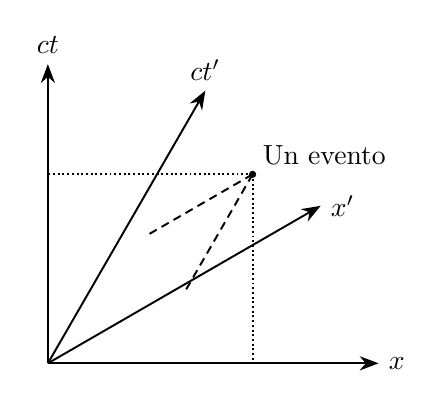
\begin{tikzpicture}[>={Stealth[length=2.4mm]}, line width=0.7pt]
  % sistema no primado (ortogonal)
  \draw[->] (0,0)--(4.2,0) node[right]{$x$};
  \draw[->] (0,0)--(0,3.8) node[above]{$ct$};
  % sistema primado (inclinado): x' a 30°, ct' a 60°
  \draw[->] (0,0)--(30:4.0) node[right]{$x'$};
  \draw[->] (0,0)--(60:4.0) node[above]{$ct'$};
  % un evento
  \coordinate (E) at (2.6,2.4);
  \fill (E) circle (1.3pt) node[above right]{Un evento};
  % proyecciones no primadas (líneas punteadas a los ejes ortogonales)
  \draw[densely dotted] (E)--(2.6,0); \draw[densely dotted] (E)--(0,2.4);
  % proyecciones primadas (paralelas a los ejes inclinados)
  \draw[densely dashed] (E)--($(E)+(60:-1.7)$);
  \draw[densely dashed] (E)--($(E)+(30:-1.55)$);
\end{tikzpicture}
\end{document}
